\chapter{Background}
The three core mechanisms used for dynamically adjusting stream processing in this thesis are Service Level Objectives (SLOs), Elasticity and Active Inference (AIF). This chapter introduces foundational concepts, essential for understanding how Active Inference
can be effectively leveraged to uphold Service Level Objectives (SLOs) in resource-constrained
edge computing environments. The first section establishes the critical role of SLOs in edge computing scenarios. The subsequent section defines the role of Elasticity in Edge Computing Systems. The penultimate section explores all of the key concepts regarding Active Inference and the Free Energy Principle. The final section discusses the principles for using AIF in distributed systems.

\section{Edge Computing and Service Level Objectives}
Edge computing refers to a distributed computing paradigm in which data processing occurs in
close proximity to the data source. This architectural shift reduces the latency and bandwidth
limitations inherent in centralized cloud computing \cite{deng_edge_2020}, while enabling real-time
analytics for latency-sensitive tasks such as autonomous driving, smart surveillance, and
industrial automation \cite{zhang_octopus_2023}.

Edge computing environments are characterized by pronounced heterogeneity \cite{furst_elastic_2018} , i.e, resource-asymmetry, vendor specifications, and usage patterns \cite{danilenka_adaptive_2025}. Devices may range from embedded computing boards to more capable edge servers, each
with distinct resource constraints in terms of CPU, memory, energy, bandwidth and especially GPU, which has become a significant factor due to increasing inference demand. When tasked with continuous stream
processing (e.g., real-time video analysis), such systems must dynamically manage
computational demands without the luxury of cloud-level resource elasticity.

To formalize quality expectations in such constrained environments, Service Level Objectives
(SLOs) are used \cite{casamayor_pujol_deepslos_2024}. SLOs define quantifiable thresholds on performance metrics, such as
response time, memory usage, or energy consumption targets \cite{danilenka_adaptive_2025}. SLOs serve as internal optimization goals \cite{danilenka_adaptive_2025} to guide system behavior under varying load conditions \cite{nastic_sloc_2020}.
For example, in a video inference pipeline, one
might define an SLO that memory usage must remain below 80\% of available capacity.

Crucially, SLOs can serve a dual role: they can be targets for optimization and/or constraints that the
system must not violate \cite{casamayor_pujol_deepslos_2024, sedlak_diffusing_2024}. In edge scenarios, where stream quality competes directly with resource availability, such as video streaming tasks \cite{sedlak_adaptive_2024}, SLO-aware control is essential \cite{sedlak_slo-aware_2025}.

\section{Elasticity in Edge Computing Systems}
Elasticity refers to a system’s ability to automatically adapt to changing workloads and resource availability. Since edge devices typically operate under fixed compute budgets, scaling hardware resources is not an option. Thus, elasticity must be achieved through intelligent control of software parameters \cite{sedlak_towards_2025}.

Sedlak et al. define elasticity in \cite{sedlak_towards_2025} along multiple axes:
\begin{itemize}
  \item \textbf{Quality Elasticity} — adjusts application-level parameters such as resolution, FPS,
or inference model complexity
  \item \textbf{Resource Elasticity} — modulates CPU, memory, or I/O usage
  \item \textbf{Cost Elasticity} — optimizes for energy efficiency or execution time.
\end{itemize}

Each elasticity action impacts both the system's SLO fulfillment and its Quality of Experience
(QoE). For instance, reducing the inference model complexity alleviates computational load but may lead to less accurate results. The key challenge lies in selecting the most appropriate elasticity action under uncertainty, while maintaining SLO compliance and maximizing QoE.

Traditional control mechanisms, such as threshold-based rules, static policies or Mache Learning approaches are not optimal to address this trade-off in dynamic environments \cite{sedlak_active_2024}. A model-based approach, capable of learning and adapting to evolving contexts, is therefore required \cite{sedlak_equilibrium_2024, danilenka_adaptive_2025}.

\section{Active Inference and the Free Energy Principle}
\subsection{The Free Energy Principle}
The Free Energy Principle (FEP), as defined in \cite{friston_free-energy_2010}, provides a unified
theory of perception, action, and learning. It posits that any self-organizing system that
maintains equilibrium with its environment over time must minimize the long-term divergence between its
internal beliefs and external sensory states \cite{friston_active_2017}. This divergence, known as
surprise, refers to the difference between what an agent predicts based on its internal model and what it observes in the environment \cite{sedlak_adaptive_2024}.

\todo{Add mathematical variable for surprse}

\subsubsection{Generative Process and Model}
Agents cannot minimize surprise directly, since the actual way that the world produces sensory data
is unknown. This process that describes the true causes for how the world generates observable
outcomes is known as the \textit{generative process} \cite{friston_free-energy_2010, smith_step-by-step_2022}. As an agent is unable to observe the ``real world``, it instead creates an internal representation of the \textit{generative process}, known as the \textit{generative model}. The \textit{generative model} serves as an approximation and is used by the agent to predict and adjust its environment according to its preferences.

\begin{figure}[htbp]
    \centering
    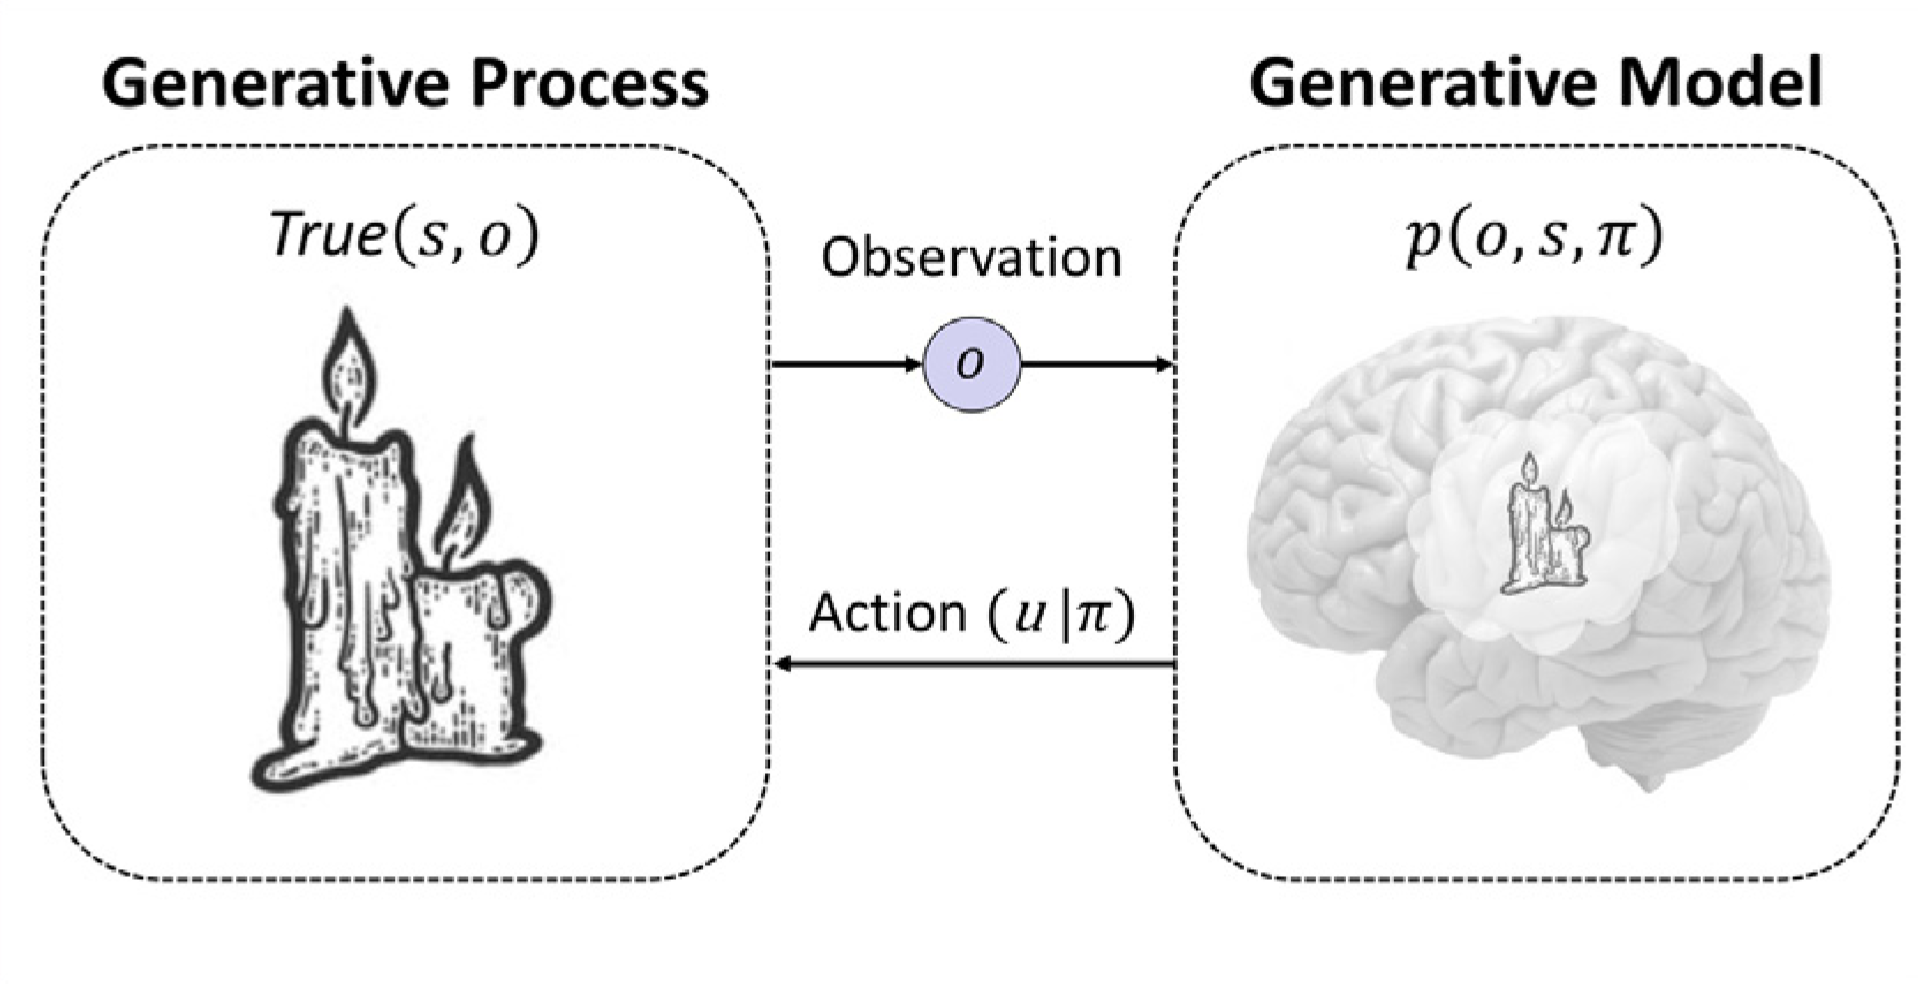
\includegraphics[width=0.8\textwidth]{img/generative-model-generative-process.png}
    \caption{Distinction and implicit coupling of generative process and the generative model. (taken from \cite{smith_step-by-step_2022})}
    \label{fig:generative-process-generative-model}
\end{figure}

When the \textit{generative process} and the \textit{generative model} differ, the agent will be ``surprised``, causing it to adjust its model closer towards the process \cite{bruineberg_free-energy_2018}. The closer the generative model is to the underlying generative process, the higher the precision of the agent's predictions is \cite{sedlak_active_2024}.

\subsubsection{Free Energy minimization}
To align the \textit{generative models} with the \textit{generative process}, the agent aims to reduce surprise to the maximum extent. A system cannot directly evaluate surprise, because this would require knowing all hidden states of the world \cite{friston_free-energy_2009}, i.e. the \textit{generative process}. Instead, an agent aims to 
minimize an upper bound \cite{smith_step-by-step_2022} known as (variational) Free Energy (FE). It captures the difference between the agent's internal representation of the world and its observations, making it a computationally feasible substitution for surprise. Therefore, by minimizing FE, agents implicitly minimize surprise \cite{friston_free-energy_2010}


FE can be expressed as the Kullback-Leibler (KL) divergence between approximate posterior probability (Q) of hidden states (x) and their exact posterior probability (P) \cite{sedlak_active_2024, sedlak_adaptive_2024,sajid_active_2021}. 
\[FE = TODO Formula and variables for Free Energy\]

 minimizing free energy minimizes KL divergence and brings the agent’s beliefs closer to the true posterior distribution \(TODO: Distribution Variables here\).

\[
\mathcal{S}(o) = -\ln{P(o)} 
\]
\[
\mathcal{O}(o) = -\ln{P(o)} 
\]

\begin{equation}
\mathcal{F} = \mathrm{KL}[Q(s) \parallel P(s|o)] - \ln P(o)
\end{equation}

\todo{check who boris cited in \cite{sedlak_adaptive_2024}}

\textbf{Variable descriptions:}
\begin{itemize}
  \item $Q(s)$: Approximate posterior (belief) over hidden states $s$, inferred by the agent.
  \item $P(o, s)$: Joint probability of observations $o$ and hidden states $s$ under the generative model.
  \item $P(o|s)$: Likelihood of observing $o$ given $s$ (encoded by matrix $\mathbf{A}$).
  \item $P(s)$: Prior over hidden states (e.g., initial state prior $\mathbf{D}$ or transition prior via $\mathbf{B}$).
  \item $\mathrm{KL}[Q(s) \parallel p(s|o)]$: Kullback--Leibler divergence between approximate posterior and true posterior.
\end{itemize}

 \subsubsection{Expected Free Energy}
To act in the world, agents must not only evaluate current states but also anticipate the outcomes of future actions. This is done via Expected Free Energy (EFE). EFE extends the concept of variational Free Energy into the future, by evaluating possible future action sequences using a policy \(\pi\). \cite{friston_active_2016}. The agent uses the EFE to decide on actions. EFE is made up of two key components \cite{friston_active_2022} % Active Inference: The Free Energy Principle in Mind, Brain, and Behavior%
\begin{enumerate}
  \item \textbf{Epistemic Value (Information Gain)} — Drives exploration by favoring actions that are expected to yield informative outcomes, improving the agent’s generative model.
  \item \textbf{Pragmatic Value} — Drives the agent to select actions that are likely to fulfill its explicit goals or preferences, i.e., it promotes exploitation.
\end{enumerate}

Together, these terms enable the agent to balance the classic exploration-exploitation tradeoff \cite{sedlak_adaptive_2024}. This dual drive allows AIF
agents to maintain SLOs while learning optimal control strategies for software parameters. \cite{lapkovskis_benchmarking_2025}.

\begin{equation}
\mathbb{G}(\pi) = \underbrace{-\mathbb{E}_{q(o, s \mid \pi)} \left[ \ln q(s \mid \pi) - \ln q(s \mid o, \pi) \right]}_{\text{information gain}} - \underbrace{\mathbb{E}_{q(o \mid \pi)} \left[ \ln p(o) \right]}_{\text{pragmatic value}}
\end{equation}

\todo{Use formula from \cite{danilenka_adaptive_2025} with DKL}

\todo{check who they cited in \cite{danilenka_adaptive_2025}}


\textbf{Variable explanations:}
\begin{itemize}
  \item $s$: Hidden States
  \item $o$: Observations
  \item $\pi$: A policy, i.e., a sequence of actions the agent may take.
  \item $q(s \mid \pi)$: Predicted posterior distribution over hidden states $s$ under policy $\pi$.
  \item $q(s \mid o, \pi)$: Updated posterior over states after observing $o$, given policy $\pi$.
  \item $q(o \mid \pi)$: Predictive distribution over future observations under policy $\pi$.
  \item $p(o)$: Preferred (prior) probability of observations, encoded as agent’s prior preferences.
\end{itemize}





\subsection{Active Inference}
Active inference (AIF) operationalizes the Free Energy Principle in artificial agents, extending it to encompass both state estimation and action selection \cite{sedlak_equilibrium_2024, lanillos_active_2021}. To implement the concepts of the Free Energy Principle, an agent maintains a \textit{generative model}, which includes the following categorical distributions \cite{heins_pymdp_2022}:

\begin{itemize}
  \item \textbf{Observation model \(P(o \mid s)\):} Defines how the hidden states produce observations and allows the agent to infer what it expects to see, given its beliefs about the world. Specifically, the likelihood model specifies the probability of an observation \(o\) given a hidden state \(s\). 
  \item \textbf{Transition model \(P(s_{t+1} \mid s_t,a_t)\):} Defines how hidden states evolve over time, depending on the actions taken by the agent. Specifically, the likelihood model explains: If the agent is in state \(s_t\) and takes action \(a_t\), what is the probability that it will end up in state \(s_{t+1}\). 
  \item \textbf{Prior preferences over observations \(P(o)\):} The agent's preferences, encoded as preferred observations (e.g., SLO fulfillment). Action selection is biased by this preference distribution, leading agents to choose actions that bring them to states that (they expect) will lead to preferred observations. It returns the numerical preference for a given observation \(o\).
  \item \textbf{Prior beliefs about hidden states \(P(s_0)\):} The initial beliefs about the environment. This is the starting point that the agent uses for inference at the first time step. It returns the probability of being in state \(s_0\).
  \item \textbf{Prior beliefs about policies: \(P(\pi)\):} Expectations about the outcomes of possible sequences. It biases the agent toward certain policies before observing anything or computing EFE. Useful for modeling habits, biases, or repetition.
\end{itemize}

\subsubsection{The Active Inference loop}
\label{sec:active-inference-loop}
To decrease EFE and consequently align the \textit{generative model} with the \textit{generative process}, the agent repeatedly engages in an action-perception loop \cite{sedlak_equilibrium_2024}. Figure \ref{fig:acive-inference-loop} provides a high-level overview. During each cycle, the agent performs three main steps \cite{heins_pymdp_2022}:
\begin{enumerate}
    \item \textbf{Perception:} Sampling an observation from the environment.
    \item \textbf{Belief updating:} Updating the agent’s beliefs about states and policies using the
observation.
    \item \textbf{Action:} Choosing and executing actions that minimize EFE, based on the agent’s posterior over policies.
\end{enumerate}

This loop is executed at regular intervals during an agent's lifetime. As Bruineberg et al. summerize in \cite{bruineberg_free-energy_2018}: ``This gives rise to a continuous feedback loop, in which what the agent does changes the environment, which changes what the agent perceives, which changes the expectations of the agent, which in turn changes what the agent does (to change the environment).``

\begin{figure}[htbp]
    \centering
    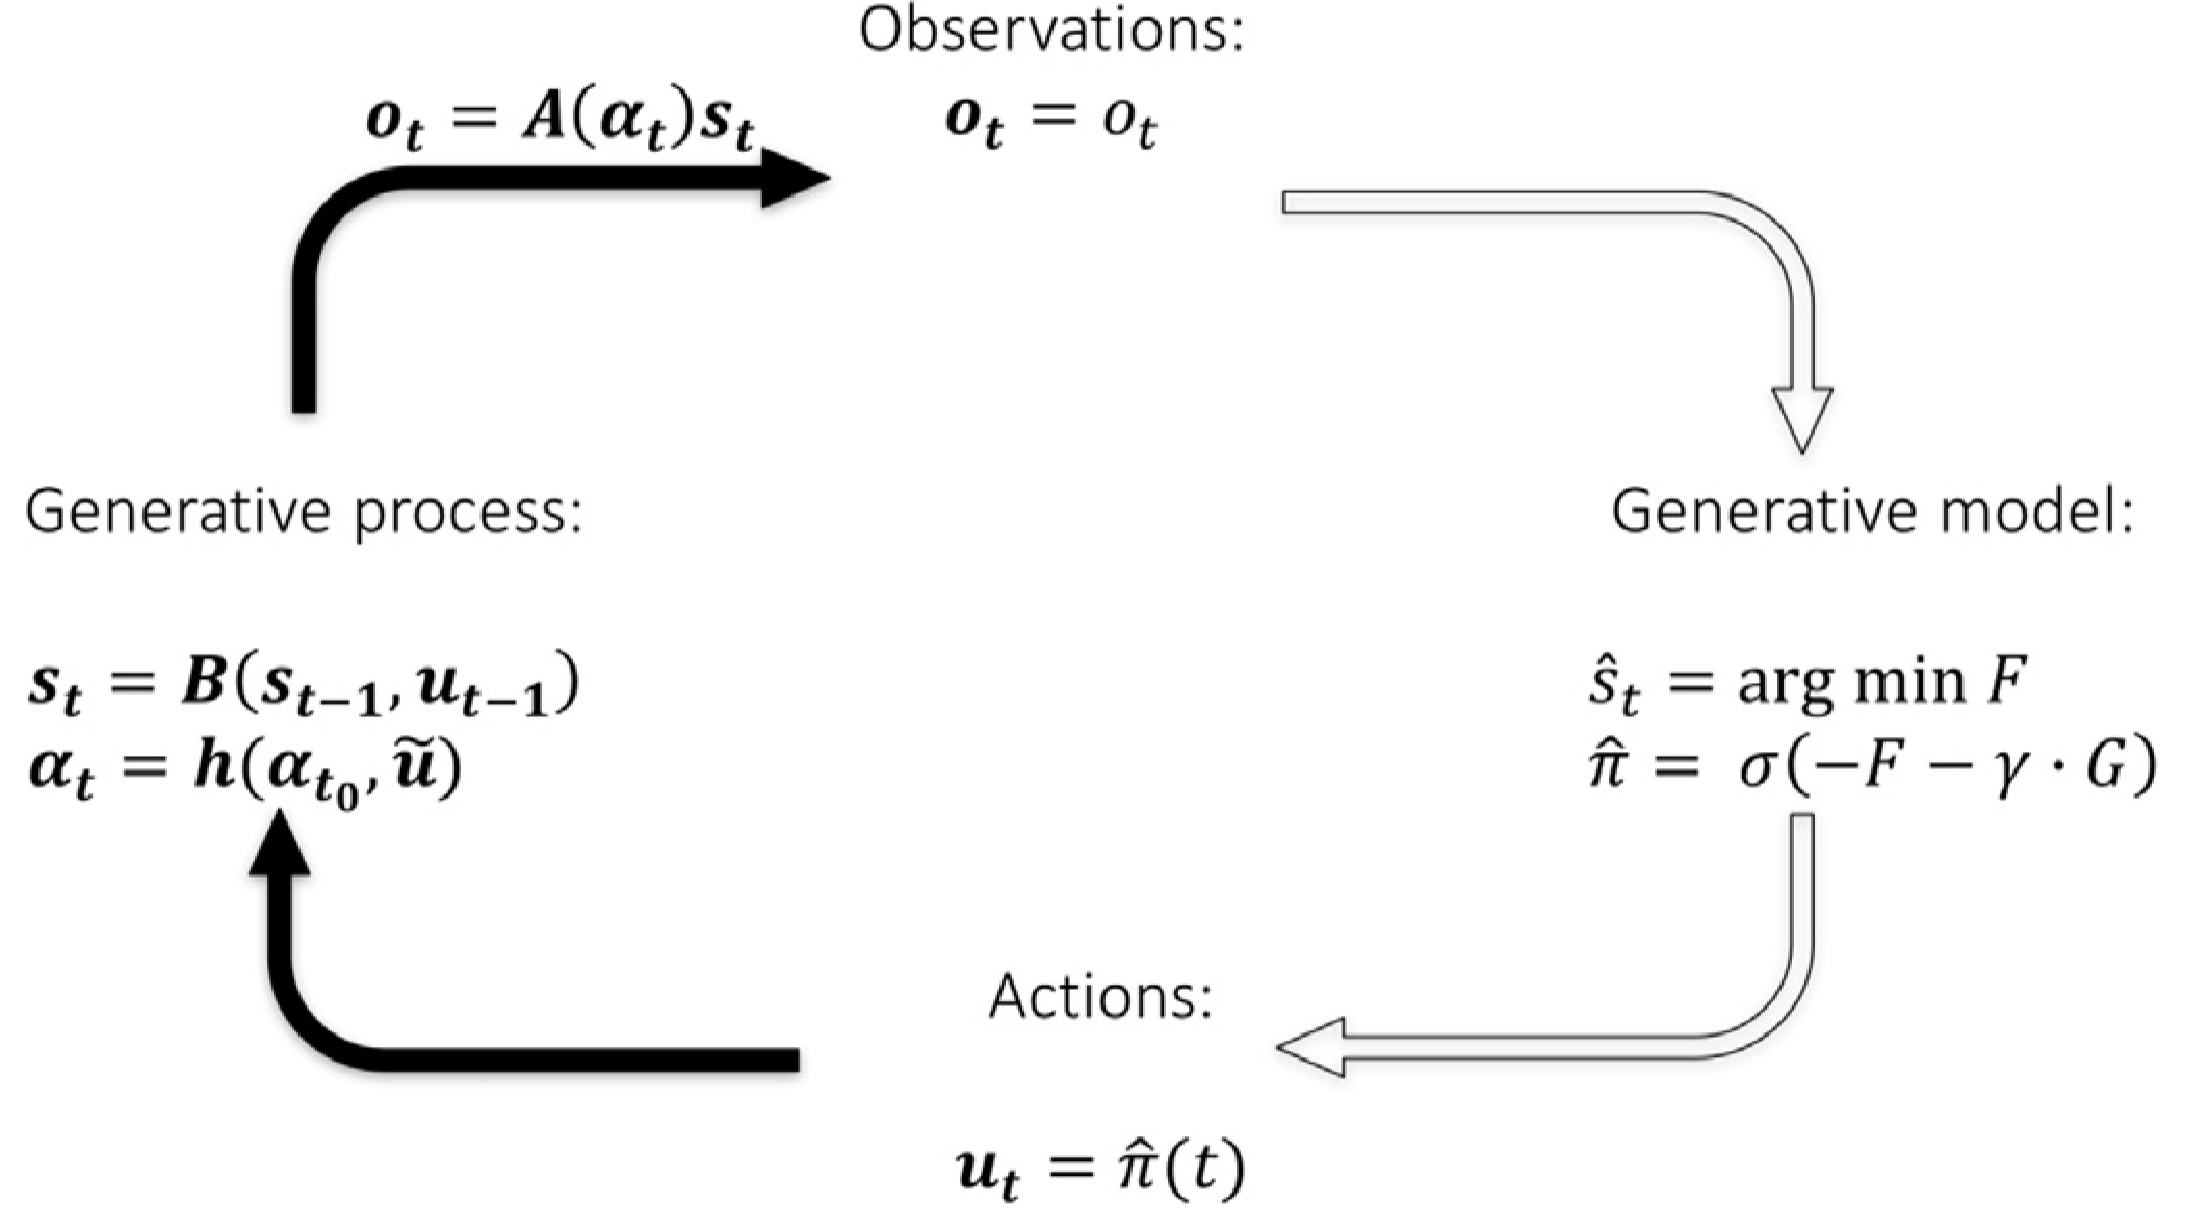
\includegraphics[width=0.8\textwidth]{img/active-inference-loop.png}
    \caption{The Active Inference loop. (taken from \cite{bruineberg_free-energy_2018})}
    \label{fig:acive-inference-loop}
\end{figure}

\section{Active Inference in Distributed Systems}
The application of active inference (AIF) to distributed systems, such as edge pipelines or multi-agent infrastructures, enables robust and interpretable control in dynamic and resource-constrained environments. Distributed systems often consist of asynchronous components with overlapping responsibilities, limited observability, and evolving workloads—conditions that challenge traditional rule-based or purely data-driven control methods. AIF addresses these challenges by equipping agents with generative models that capture the causal relationships between system parameters (e.g., processing configurations) and observed outcomes (e.g., SLO satisfaction). By interacting with the environment and updating beliefs, agents learn how their actions affect system behavior. This iterative action-perception cycle allows agents to adapt to their environment during their lifetime. As Sedlak et al. note in \cite{sedlak_active_2024}, “The agent used causal knowledge to gradually develop an understanding of how its actions are related to requirements fulfillment, and which configurations to favor”.

In distributed edge pipelines, AIF agents can operate locally, managing a single node or service, or hierarchically, coordinating across components to optimize system-level objectives. In both cases, adaptation is driven by minimizing EFE. This balances two goals: maximizing the probability of fulfilling preferences (i.e., SLOs and QoE goals) and reducing uncertainty about the system \cite{friston_free-energy_2010, lanillos_active_2021}. 

This thesis implements a single-agent variant of this framework: an AIF controller monitors the global state of a distributed stream processing pipeline and dynamically adjusts elasticity parameters that impact the quality of the system's output. The agent intervenes when SLOs (e.g., memory constraints) approach critical levels and selects adaptations that restore compliance while improving its generative model \cite{sedlak_equilibrium_2024}.

Although focused on a centralized AIF controller, the underlying framework is inherently extensible to multi-agent settings, where distributed agents can share beliefs or synchronize generative models. Prior work has demonstrated how such agents can collaboratively manage resources and task assignments in real-time systems while maintaining local autonomy and decentralized control \cite{sedlak_slo-aware_2025}. Such concepts will be discussed in chapter\ref{chap:related-work}
